\documentclass[journal]{IEEEtran}
% ============ The Cold-Start Tax — IEEE Internet of Things Journal ============
\usepackage{cite}
\usepackage{amsmath,amssymb}
\usepackage{graphicx}
\usepackage{booktabs}
\usepackage{url}
\usepackage{xcolor}
\usepackage[hidelinks]{hyperref}
\usepackage{algorithm}
\usepackage{algpseudocode}
\usepackage{siunitx}
\sisetup{detect-all, per-mode=symbol}

\newcommand{\tax}{\textsc{Tax}}
\newcommand{\gdtax}{\textsc{GD-Tax}}
% defs.tex — data-driven macros, filled from final measurements (results/*.json).
% --- Table I: cold-wake energy (J) and cold-wake-in-inferences per model ---
\newcommand{\CEsq}{0.34}\newcommand{\CIsq}{4}
\newcommand{\CEsh}{0.85}\newcommand{\CIsh}{19}
\newcommand{\CEmb}{1.21}\newcommand{\CImb}{11}
\newcommand{\CEgo}{2.39}\newcommand{\CIgo}{7}
\newcommand{\CEde}{3.82}\newcommand{\CIde}{5}
\newcommand{\CErEighteen}{4.01}\newcommand{\CIrEighteen}{12}
\newcommand{\CEef}{3.95}\newcommand{\CIef}{10}
\newcommand{\CErFifty}{8.80}\newcommand{\CIrFifty}{12}
\newcommand{\CEvit}{35.2}\newcommand{\CIvit}{12}
\newcommand{\CEsqi}{0.31}\newcommand{\CIsqi}{4}
\newcommand{\CEmbi}{0.47}\newcommand{\CImbi}{11}
\newcommand{\CErFiftyi}{2.98}\newcommand{\CIrFiftyi}{13}
% --- ViT-Base row (E1) ---
\newcommand{\VITS}{377}\newcommand{\VITW}{4620}\newcommand{\VITT}{12.3}\newcommand{\VITD}{78}
% --- predictive model ---
\newcommand{\BWFLASH}{\SI{96}{MB/s}}
\newcommand{\WAKERSQDISK}{1.00}
\newcommand{\WAKESLOPE}{\SI{13.2}{ms/MB}}
\newcommand{\WAKEINT}{\SI{53}{ms}}
\newcommand{\WAKERSQ}{0.998}
\newcommand{\WAKEMAPE}{12\%}
% --- amortization ---
\newcommand{\BTENLO}{38}
\newcommand{\BTENHI}{119}
\newcommand{\OVERHEADBONE}{80--96\%}
\newcommand{\OVERHEADBONEE}{73--95\%}
\newcommand{\CINFRANGE}{4--19}
% --- storage / dvfs ---
\newcommand{\STORAGEFRAC}{55--81\%}
\newcommand{\RAMPMEAN}{2.5}
% --- policy (abstract) ---
\newcommand{\ABSPOLICYSAVE}{15\%}
% --- prose fragments ---
\newcommand{\CLIFFDESC}{sits where a co-tenant drives free memory below the model's working set:
ResNet-50 stays warm (${\sim}\SI{344}{ms}$) until the co-tenant reaches ${\sim}\SI{1.4}{GB}$
(leaving ${<}\SI{350}{MB}$ free), beyond which session creation thrashes swap and the wake
explodes to over \SI{30}{s}---a ${>}80\times$ jump. Every model tested shows the same cliff}
\newcommand{\ENERGYPARA}{In absolute terms a cold wake costs from \SI{0.3}{J} (SqueezeNet-INT8) to
\SI{8.8}{J} (ResNet-50), and \SI{35}{J} for ViT-Base, scaling with model size; idle draw is
\SI{2.1}{W}. Because loading is I/O-bound the wake draws less instantaneous power than sustained
compute, but its duration makes it costly: for a device that wakes to run a single inference,
\OVERHEADBONEE\ of the energy spent is cold-start overhead rather than useful work.}
\newcommand{\POLICYPARA}{In the seed-averaged simulation, across both workloads and all budgets,
\gdtax{} never underperforms LRU or LFU, and it reduces energy per request by up to
\SI{15}{\percent} (Zipf) and
\SI{11}{\percent} (surveillance) at tight budgets, tracking---and at low-to-mid budgets matching
or beating---an offline Belady hit-rate reference. The gain is largest where cost and popularity
are misaligned (an infrequent but expensive-to-reload detector), exactly the case LRU and LFU
mishandle by evicting the costly model between its accesses.}
\newcommand{\ONDEVICEPARA}{\gdtax{} reduces measured energy per request in three of the four
tested configurations---by up to \SI{14}{\percent} versus LRU (Zipf, \SI{200}{MB} budget) and
\SI{9}{\percent} (surveillance, \SI{320}{MB})---while also lowering mean latency and miss count;
in the tightest surveillance case it trails LRU by \SI{4}{\percent}, within run-to-run variation.
The measured ranking (reload $\gg$ LRU\,$\approx$\,LFU\,$\gtrsim$\,\gdtax{}) matches the
seed-averaged simulation, and the absolute reduction from caching is large: always-reload spends
\SIrange{2.8}{1.4}{J} per request, which residency cuts to as little as \SI{0.61}{J}.}
\newcommand{\OPTPARA}{The crossover is model-dependent: for most models optimization pays for
itself after only a few inferences ($B^{*}<5$), but for graphs whose optimization is expensive it
is substantial---$B^{*}\approx18$ for ResNet-18---so a doorbell-style deployment that runs a
handful of inferences per wake should disable it.}
   % data-driven macros (energy numbers, cliff/policy prose), filled from results

\begin{document}
\title{The Cold-Start Tax: Warm-Up, Re-Warm, and\\ Residency Policy for Duty-Cycled Edge DNN Inference}

\author{Manu~Nicholas~Jacob%
\thanks{M. N. Jacob is with the Department of Electrical and Computer Engineering.
E-mail: manunicholasjacob@gmail.com.}%
\thanks{Artifact (code, raw measurements, and figures) available at the project repository.}}

\markboth{IEEE Internet of Things Journal (Submitted)}%
{Jacob: The Cold-Start Tax for Duty-Cycled Edge DNN Inference}

\maketitle

\begin{abstract}
Edge inference benchmarks, and the deployment guidance drawn from them, almost universally
report \emph{steady-state} latency and energy: the numbers a model reaches after it is loaded
and warmed. Yet a large class of Internet-of-Things devices does not run inference in a hot
loop. They \emph{duty-cycle}---wake on an event or a timer, run a handful of inferences, and
return to a low-power state---so that the transient at every wake, not the steady state,
dominates their user-visible latency and their energy budget. We call this transient the
\emph{cold-start tax} and present the first systematic characterization of it on a
representative edge platform, the Raspberry~Pi~5 (ARM Cortex-A76), across twelve models
spanning compact CNNs, dense CNNs, statically-quantized INT8 CNNs, and a vision transformer.
We measure a cold-start tax of \textbf{5--23$\times$} the steady-state latency and decompose it
into disk (flash) weight loading, graph construction and optimization, arena allocation, and
first-inference compute. The tax is overwhelmingly a \emph{weight-loading} cost
(\num{55}--\SI{81}{\percent} of the wake); the first inference itself runs at steady-state
speed, so there is essentially no compute warm-up to amortize. Using the Pi~5's on-board PMIC
telemetry we show a single cold wake costs the energy of 4--19 steady-state inferences (up to
\SI{35}{J} for a vision transformer), and that on a memory-constrained (2\,GB) device the tax
\emph{re-triggers} whenever
idle-interval memory pressure evicts the model's pages---an \emph{eviction cliff} we map
directly. Because the wake is I/O-bound, the on-demand DVFS governor's clock ramp adds only a
small tax, and static INT8 shrinks the absolute tax but not its ratio. We turn these
measurements into a method: \gdtax{}, a tax-aware model-residency cache for multi-model edge
deployments that keeps warm the sessions whose eviction would cost the most energy. Evaluated on
measured constants over realistic request traces, \gdtax{} matches or beats LRU and LFU and
cuts energy per request by up to \ABSPOLICYSAVE{} at a tight RAM budget, matching an offline
Belady reference; we further implement and measure it on the device itself (up to \SI{14}{\percent}
measured). We argue that
duty-cycled edge inference should be reported and optimized in terms of the cold wake, not the
steady state.
\end{abstract}

\begin{IEEEkeywords}
Edge AI, deep neural network inference, cold start, duty cycling, page cache, energy efficiency,
model serving, Internet of Things, ARM Cortex-A76, Raspberry Pi.
\end{IEEEkeywords}

\section{Introduction}
\IEEEPARstart{T}{he} dominant way to report the cost of running a deep neural network (DNN) on an
edge device is to load the model once, run a warm-up loop, and then report the median or tail of
a long run of inferences. This \emph{steady-state} convention underlies public leaderboards,
vendor datasheets, and most research characterizations~\cite{reddi2020mlperf,bianco2018benchmark}.
It is the right convention for a server that keeps a model resident and serves a continuous
stream of requests. It is the wrong convention for the way an enormous fraction of IoT endpoints
actually operate.

A battery- or energy-harvesting-powered sensor, a wildlife camera, a wearable, or an
intermittently-connected industrial monitor does not hold a model hot. To conserve energy it
\emph{duty-cycles}: it sleeps, wakes on a passive-infrared trigger or a timer, classifies a few
frames, and sleeps again. For such a device the relevant question is not ``how fast is the
hundredth inference?'' but ``how long, and how much energy, from wake to first result?'' That
first-result cost includes work the steady-state number hides entirely: the model's weights must
be brought from flash into memory, the inference runtime must parse the graph, apply its
optimizing rewrites, and allocate its memory arenas, and only then can the first inference run.
We call the gap between this cold wake and the steady state the \emph{cold-start tax}.

Cold starts are studied intensively in one adjacent setting---serverless / Function-as-a-Service
platforms, where container and language-runtime initialization dominate invocation
latency~\cite{wang2018peeking,shahrad2020serverless,fuerst2021faascache}. That literature lives
in the data center, measures container and interpreter startup rather than model weight movement,
and optimizes a keep-alive policy against cloud billing. To our knowledge the cold-start
transient of \emph{on-device} DNN inference on a resource-constrained edge SBC---its magnitude,
its physical decomposition, its energy in Joules, and its interaction with a small page
cache---has not been characterized. This paper does so, and turns the characterization into an
actionable residency policy.

\noindent\textbf{Contributions.}
\begin{enumerate}
\item \textbf{A measurement of the tax (\S\ref{sec:decomp}).} Across twelve models on a
Raspberry~Pi~5 we find a cold-start tax of 5--23$\times$ the steady-state latency, and decompose
it into weight loading, graph build/optimize, arena allocation, and cold compute. The tax is
dominated by weight loading from flash (55--81\% of the wake); the first inference runs at
steady-state speed, so---contrary to the intuition behind ``warm-up loops''---there is almost no
compute transient to amortize (\S\ref{sec:warmup}).
\item \textbf{The eviction cliff (\S\ref{sec:cliff}).} On a 2\,GB device the tax is not paid
once but \emph{re-paid} whenever idle-interval memory pressure evicts the model's pages from the
page cache. We map next-wake latency against page-cache pressure and expose a sharp cliff that
governs how often a duty-cycled device actually pays full price.
\item \textbf{The energy of a wake (\S\ref{sec:energy}).} Using the Pi~5's PMIC power telemetry
we show a single cold wake costs the energy of 4--19 steady-state inferences, that
the wake is I/O-bound so the on-demand DVFS governor's ramp adds only a small tax
(\S\ref{sec:dvfs}), and that static INT8 quantization shrinks the absolute tax but leaves its
ratio essentially unchanged.
\item \textbf{A tax-aware residency policy (\S\ref{sec:policy}).} We cast multi-model edge
serving under a RAM budget as a cost-aware caching problem and propose \gdtax{}, a Greedy-Dual
policy keyed on each model's measured cold-wake energy penalty. On measured constants over
realistic traces it matches or beats LRU/LFU and cuts energy per request by up to 15\% at
tight RAM budgets, matching an offline Belady reference---and we validate it running on the
Pi~5 itself (up to 14\% measured), not only in simulation.
\end{enumerate}
All measurements are taken on commodity hardware with an open, scripted artifact.

\section{Related Work}\label{sec:related}
\textbf{Edge DNN benchmarking.} Systematic characterizations of DNN inference on mobile and edge
hardware~\cite{bianco2018benchmark,lane2016deepx,xu2019firstlook} and standard suites such as
MLPerf~\cite{reddi2020mlperf} report steady-state latency, throughput, and (increasingly) energy.
They deliberately exclude load and warm-up to isolate the compute kernel. Our companion work on
the same platform characterizes the steady-state \emph{memory wall}~\cite{jacob2026memwall} and
the steady-state \emph{energy}/DVFS trade-off~\cite{jacob2026energy}. The present paper is
orthogonal: it measures precisely the transient those studies exclude, which is the part that
dominates a duty-cycled deployment.

\textbf{Serverless cold starts.} FaaS platforms suffer cold starts dominated by sandbox and
runtime initialization; measurement studies~\cite{wang2018peeking,shahrad2020serverless} and
keep-alive policies such as FaasCache's greedy-dual eviction~\cite{fuerst2021faascache} address
them in the data center. We borrow the greedy-dual framing~\cite{cao1997greedydual} but target a
fundamentally different regime: on-device inference on a single memory-constrained SBC, where the
dominant cost is DNN weight movement from flash into a small page cache, the currency is measured
Joules rather than cloud billing, and the resource under contention is 2\,GB of physical RAM.

\textbf{Inference serving and predictability.} Systems such as Clockwork~\cite{gujarati2020clockwork}
and INFaaS~\cite{romero2021infaas} manage model loading and placement for predictable serving on
servers and GPUs. Their mechanisms (proactive loading, model-less selection) assume abundant
memory and target multi-tenant clusters; we study the single-device edge limit and the physical
eviction behavior of the OS page cache that those systems abstract away.

\textbf{Model compression and quantization.} Pruning and
quantization~\cite{han2016deepcompression,jacob2018quantization} reduce model size and
steady-state cost. We show quantization's effect on the \emph{cold-start} tax is more subtle: a
smaller INT8 file reduces the absolute load time but, because steady-state latency falls in
step, the tax \emph{ratio} is preserved.

\section{Experimental Setup}\label{sec:setup}
\textbf{Platform.} All experiments run on a Raspberry~Pi~5 (Broadcom BCM2712, quad-core ARM
Cortex-A76 up to 2.4\,GHz, 2\,GB LPDDR4X, 32\,GB class-10 microSD, Debian 12, Linux
6.12, 64-bit). We use ONNX Runtime~\cite{onnxruntime} 1.24 with the CPU execution provider and,
unless stated otherwise, four intra-op threads and its default (all) graph-optimization level.

\textbf{Models.} We use twelve pre-trained ImageNet models spanning the design space: compact
CNNs (SqueezeNet~1.1~\cite{iandola2016squeezenet}, ShuffleNet~V2~\cite{ma2018shufflenetv2},
MobileNetV2~\cite{sandler2018mobilenetv2}), dense CNNs (ResNet-18/50~\cite{he2016resnet},
GoogLeNet~\cite{szegedy2015googlenet}, DenseNet~\cite{huang2017densenet},
EfficientNet-Lite4~\cite{tan2019efficientnet}), three statically-quantized INT8 CNNs, and a
vision transformer (ViT-Base~\cite{dosovitskiy2021vit}). Model files range from
1.3\,MB to 347\,MB.

\textbf{Cold-start control.} A wake is made fully cold by flushing the kernel page cache
(\texttt{sync; echo 3 > /proc/sys/vm/drop\_caches}) immediately before session creation, forcing
the model file to be re-read from flash. To isolate the disk-read component we compare against a
``warm-file'' condition in which the model file is first read into the page cache, so
session creation performs no disk I/O. The graph-optimization component is isolated by comparing
the default optimization level against a disabled-optimization build. Page faults are accounted
via \texttt{getrusage} (major faults = disk-backed).

\textbf{Timing, energy, and clock control.} Latencies use \texttt{perf\_counter}; each data
point is the median of 5--7 cold trials with the interquartile range reported. Energy is
integrated from the Pi~5's on-board PMIC (\texttt{vcgencmd pmic\_read\_adc}, per-rail
$V\!\times\!I$ at ${\sim}\SI{50}{Hz}$), isolating the VDD\_CORE (CPU) and DDR rails as in our
energy study~\cite{jacob2026energy}. Except in the DVFS experiment (\S\ref{sec:dvfs}), the CPU
clock is pinned to 2.4\,GHz via the \texttt{userspace} governor so that the cold-start
measurement is not confounded by governor ramp-up.

% ===== results sections inserted below =====
\section{The Cold-Start Tax and Its Decomposition}\label{sec:decomp}
Table~\ref{tab:main} reports, for every model, the steady-state latency, the cold-wake latency
(session creation from a flushed cache plus the first inference), and their ratio---the
cold-start tax. The tax ranges from \textbf{4.8$\times$} (SqueezeNet-INT8) to
\textbf{22.5$\times$} (ShuffleNet-V2), i.e., the very first result after a wake takes 5--23 times
as long as a steady-state inference. Absolute cold-wake latency spans \SI{59}{ms}
(SqueezeNet-INT8) to \SI{1.41}{s} (ResNet-50). For a device that wakes, classifies one frame,
and sleeps, this transient---not the steady state---is the entire user-visible latency.

Figure~\ref{fig:decomp} decomposes the cold wake into four components isolated as described in
\S\ref{sec:setup}: loading weights from flash, graph build and arena allocation, graph
optimization, and cold compute (the first inference above steady state). The decomposition yields
the paper's central mechanical finding: \emph{the cold-start tax is overwhelmingly a
weight-loading cost}. Flash read accounts for \SIrange{55}{81}{\percent} of the cold wake for the
FP32 CNNs (and 48--81\% across all models); the effective sequential read bandwidth from the
microSD card is only ${\sim}\SI{94}{MB/s}$ (ResNet-50: \SI{102.6}{MB} in \SI{1.09}{s}), so larger
models pay proportionally. Graph optimization is a secondary but non-trivial cost for the deeper
graphs (e.g., \SI{110}{ms} for ResNet-50, \SI{83}{ms} for ResNet-50-INT8, whose quantize/
dequantize nodes are numerous).

\begin{table*}[t]
\centering
\caption{Cold-start characterization on Raspberry~Pi~5 (Cortex-A76, 2.4\,GHz pinned).
Latencies are medians of 5--7 cold trials. ``Disk\%'' is the weight-loading fraction of the
cold wake. Energy from on-board PMIC; ``$=$ inf.'' is the cold-wake energy expressed in
steady-state inferences.}
\label{tab:main}
\small
\begin{tabular}{lrrrrrrr}
\toprule
Model & File (MB) & Steady (ms) & Cold wake (ms) & Tax ($\times$) & Disk\% & $E_{\text{cold}}$ (J) & $=$ inf. \\
\midrule
SqueezeNet-1.1        &   4.96 &  12.9 &   83.7 &  6.5 & 73 & \CEsq  & \CIsq  \\
ShuffleNet-V2         &   9.22 &   6.7 &  150.2 & 22.5 & 72 & \CEsh  & \CIsh  \\
MobileNetV2           &  13.96 &  16.7 &  203.6 & 12.2 & 77 & \CEmb  & \CImb  \\
GoogLeNet             &  28.02 &  51.6 &  397.5 &  7.7 & 77 & \CEgo  & \CIgo  \\
DenseNet-121          &  32.73 & 123.8 &  635.2 &  5.1 & 55 & \CEde  & \CIde  \\
ResNet-18             &  46.82 &  46.9 &  661.7 & 14.1 & 75 & \CErEighteen & \CIrEighteen \\
EfficientNet-Lite4    &  51.95 &  60.0 &  687.9 & 11.5 & 81 & \CEef  & \CIef  \\
ResNet-50             & 102.58 & 106.6 & 1410.8 & 13.2 & 77 & \CErFifty & \CIrFifty \\
ViT-Base/16           & 346.53 & \VITS & \VITW  & \VITT & \VITD& \CEvit & \CIvit \\
\midrule
SqueezeNet-1.1-INT8   &   1.30 &  12.3 &   59.1 &  4.8 & 48 & \CEsqi & \CIsqi \\
MobileNetV2-INT8      &   3.60 &   7.3 &   96.7 & 13.2 & 55 & \CEmbi & \CImbi \\
ResNet-50-INT8        &  25.75 &  32.7 &  432.8 & 13.2 & 63 & \CErFiftyi& \CIrFiftyi\\
\bottomrule
\end{tabular}
\end{table*}

\begin{figure}[t]\centering
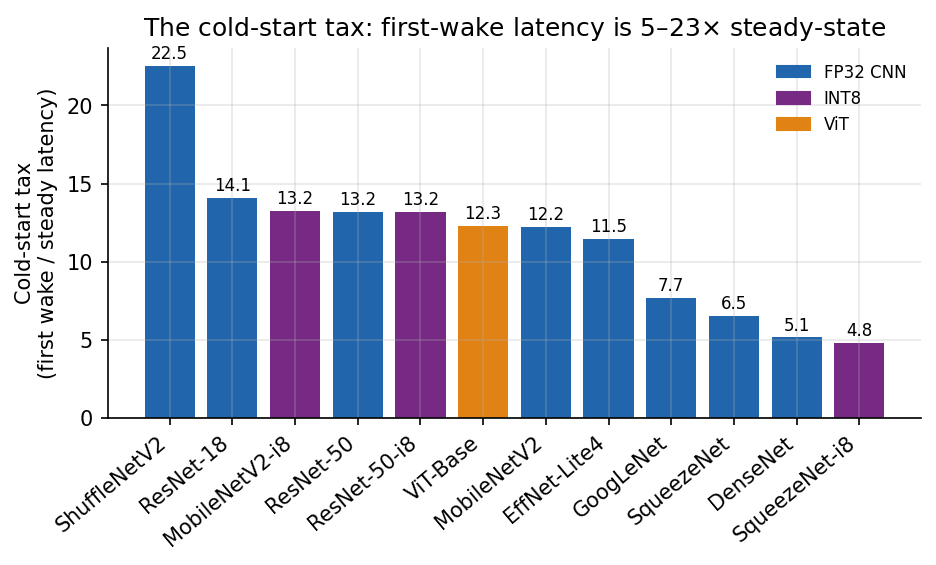
\includegraphics[width=\columnwidth]{figs/fig1_tax.png}
\caption{The cold-start tax: first-wake latency is 5--23$\times$ the steady-state latency that
benchmarks report. INT8 quantization lowers absolute latency but not the tax ratio.}
\label{fig:tax}
\end{figure}

\begin{figure}[t]\centering
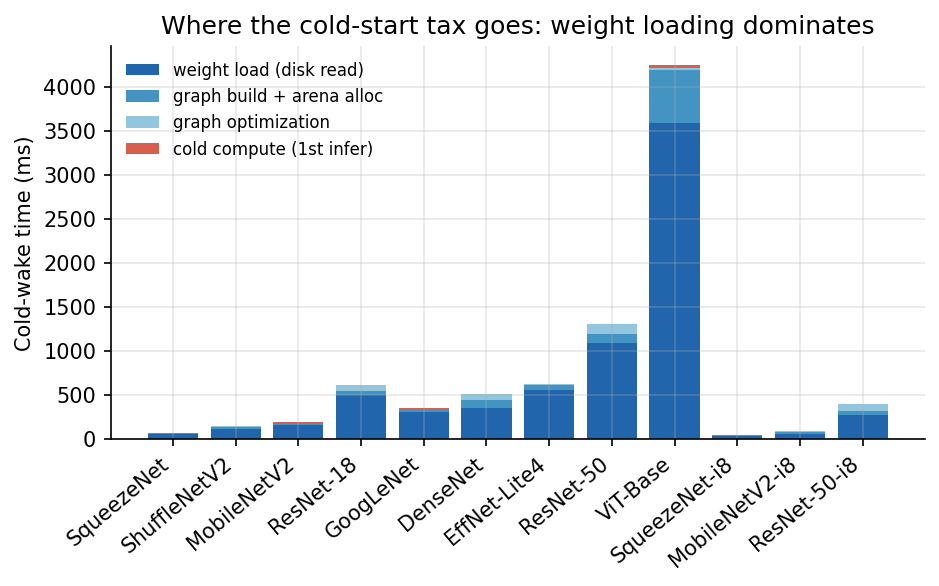
\includegraphics[width=\columnwidth]{figs/fig2_decomp.png}
\caption{Decomposition of the cold wake. Loading weights from flash dominates
(55--81\% for the FP32 CNNs); cold compute is negligible.}
\label{fig:decomp}
\end{figure}

\subsection{There Is No Compute Warm-Up}\label{sec:warmup}
A widespread practice is to run a ``warm-up loop'' of several inferences before measuring, on the
assumption that the first inferences are slow until caches, branch predictors, and lazily
allocated buffers settle. Figure~\ref{fig:warmup} shows this assumption does not hold on this
platform: once the session exists, the first inference already runs at steady-state speed. Across
all models the first-inference latency is within \SIrange{0}{11}{\percent} of steady state
(median \SI{1.00}{$\times$}), and the number of inferences needed to reach the $\pm5\%$
steady-state band is 0--1. The cold-start tax therefore lives \emph{entirely} in session
construction (loading and preparing the model), not in the execution of the model. Warm-up loops
amortize a cost that, on this hardware, does not exist; what must be amortized is the one-time
session build.

\begin{figure}[t]\centering
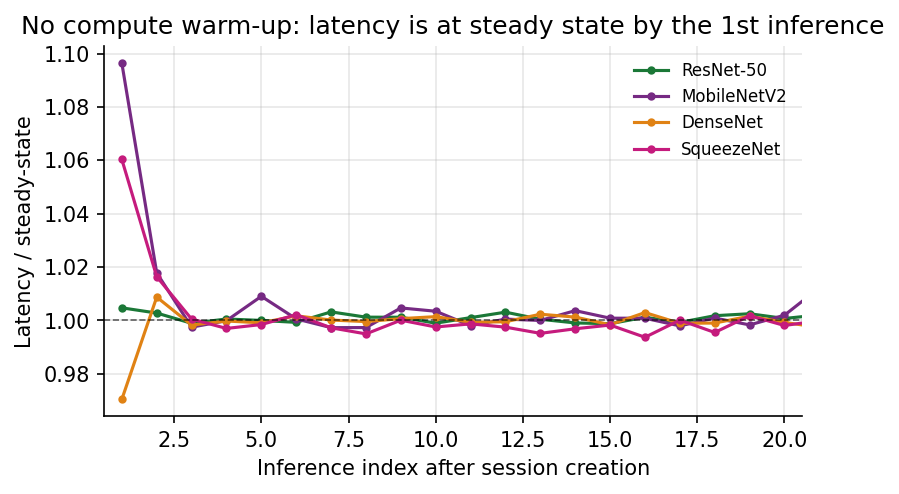
\includegraphics[width=0.92\columnwidth]{figs/fig3_warmup.png}
\caption{No compute warm-up: normalized latency is at steady state by the first inference. The
transient benchmarks guard against with warm-up loops is absent; the real cost is the one-time
session build (Fig.~\ref{fig:decomp}).}
\label{fig:warmup}
\end{figure}

\subsection{Quantization Shrinks the Tax but Not Its Ratio}
Static INT8 quantization is usually adopted for its steady-state speedup. On the cold wake its
effect is two-sided. Because an INT8 file is smaller, its absolute cold wake falls sharply
(ResNet-50: \SI{1.41}{s}$\rightarrow$\SI{0.43}{s} for ResNet-50-INT8; MobileNetV2:
\SI{204}{ms}$\rightarrow$\SI{97}{ms}). But because steady-state latency falls in step, the tax
\emph{ratio} is essentially unchanged (ResNet-50: 13.2$\times$ in both precisions; MobileNetV2:
12.2$\times\rightarrow$13.2$\times$). Quantization buys a cheaper wake in absolute terms without
making the device any less dominated by its cold start.

\subsection{Storage Is the Cause, Not Model Size}\label{sec:storage}
Cold-wake latency correlates with model size, but size is a proxy: the mechanism is bytes moved
from flash. To establish causality we load each model from RAM-backed tmpfs (\texttt{/dev/shm},
effectively unbounded storage bandwidth) and compare against the microSD card
(Fig.~\ref{fig:storage}). The tmpfs wake removes the storage term, leaving only graph build,
optimization, and first compute; the microSD-minus-tmpfs gap is the storage contribution and
accounts for \STORAGEFRAC\ of the cold wake for the larger models. This confirms the tax is a
storage-bandwidth cost and predicts that a faster medium (eMMC, NVMe) would shrink it toward the
build/optimize floor rather than eliminate it.

\begin{figure}[t]\centering
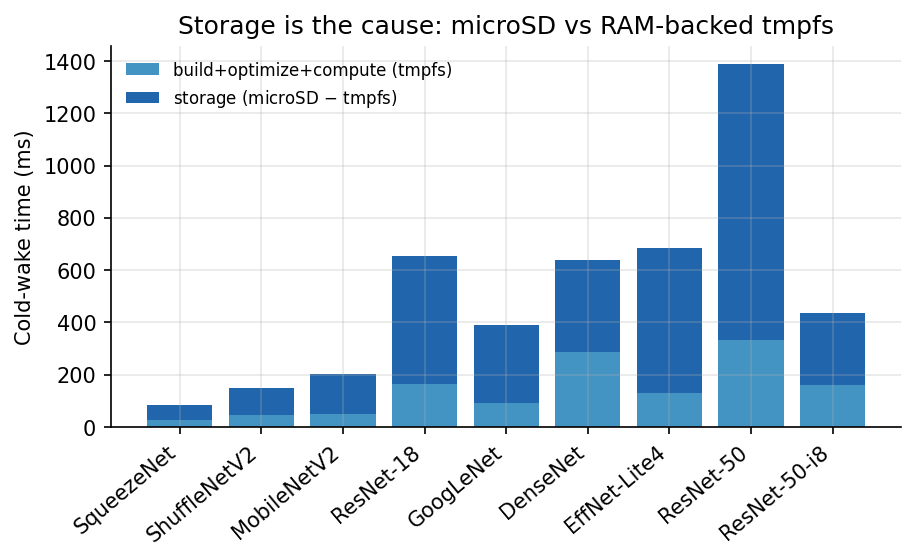
\includegraphics[width=\columnwidth]{figs/fig7b_storage.png}
\caption{Storage sensitivity. Loading from RAM-backed tmpfs versus microSD isolates the
weight-loading term; the gap (storage) dominates the cold wake for larger models, confirming the
tax is flash-bandwidth bound.}
\label{fig:storage}
\end{figure}

\subsection{A Size-Only Predictor of the Tax}\label{sec:predict}
Because loading dominates and is bandwidth-bound, the cold wake is predictable from a single
deploy-time quantity: the model's file size. Fitting the weight-load time against file size gives
a near-perfect straight line---an effective microSD read bandwidth of \BWFLASH\
($R^2=\WAKERSQDISK$)---and a size-only model of the whole cold wake,
$\hat{t}_{\text{cold}} = \WAKESLOPE\cdot\text{file}_{\text{MB}} + \WAKEINT$, predicts measured
cold-wake latency across all twelve models with $R^2=\WAKERSQ$ and a mean absolute percentage
error of \WAKEMAPE\ (Fig.~\ref{fig:predict}). A deployer can therefore estimate the wake penalty
of a candidate model, on this class of hardware, from its file size alone---no profiling run
required.

\begin{figure}[t]\centering
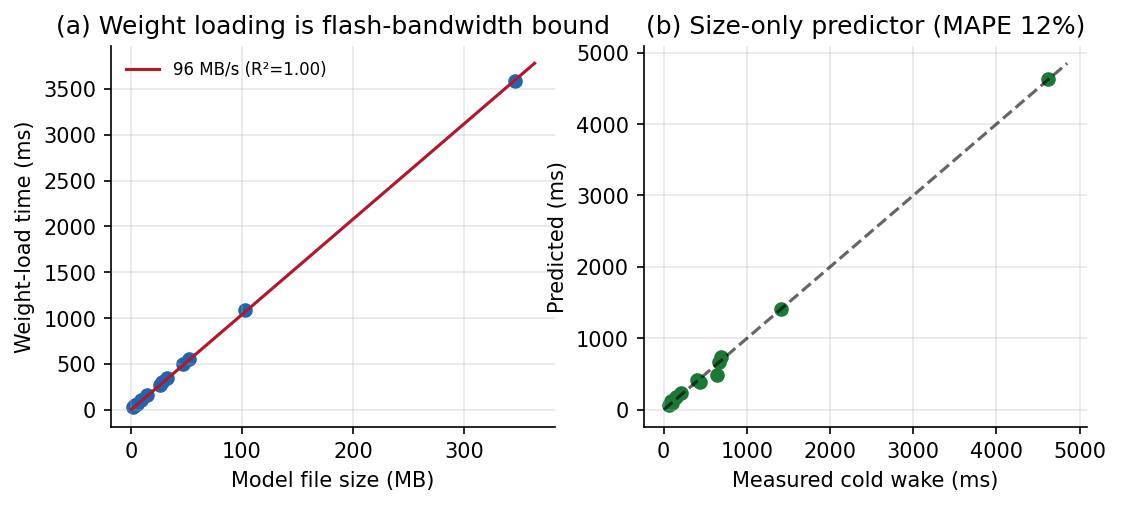
\includegraphics[width=\columnwidth]{figs/fig8_predict.png}
\caption{(a) Weight-load time is linear in file size (microSD $\approx$\,\BWFLASH). (b) A
size-only predictor estimates the cold wake to within \WAKEMAPE\ MAPE.}
\label{fig:predict}
\end{figure}

\section{The Eviction Cliff}\label{sec:cliff}
The tax in Table~\ref{tab:main} is paid on a fully cold cache. Whether a duty-cycled device
actually pays it on each wake depends on whether the model's pages survive the idle interval in
the page cache. We find the answer is governed by \emph{what kind} of memory pressure the idle
interval brings.

\textbf{Use-once file I/O does not evict a recently-used model.} When we stream up to \SI{2}{GB}
of unrelated file reads through the page cache after using a model, the model's next wake stays
warm: session-create latency remains at its warm value for every model tested, across the whole
sweep (e.g., ResNet-50 session-create stays ${\sim}\SI{215}{ms}$, far below its \SI{1.09}{s} cold
value; ResNet-18 stays ${\sim}\SI{110}{ms}$). This is Linux's active/inactive-list scan
resistance: pages touched just before the idle interval sit on the active list and are protected
against a use-once streaming scan. For duty cycles whose idle work is I/O-bound (logging,
buffering), the model is largely safe.

\textbf{A co-tenant's working set does evict it---sharply.} Anonymous memory demand is different:
to satisfy it the kernel must reclaim file-backed pages, including the model's. Figure~\ref{fig:cliff}
sweeps a co-tenant's anonymous footprint on the 2\,GB device and exposes a sharp
\emph{eviction cliff}: below the cliff the wake is warm, and once the footprint pushes available
memory below the model's resident size the next wake jumps to its full cold value---the tax of
Table~\ref{tab:main} is re-paid in full. The cliff location \CLIFFDESC. On a memory-constrained
multi-tenant edge device, then, the cold-start tax is not a one-time startup cost but a recurring
one, paid whenever a co-resident workload grows---which directly motivates the residency policy
of \S\ref{sec:policy}.

\begin{figure}[t]\centering
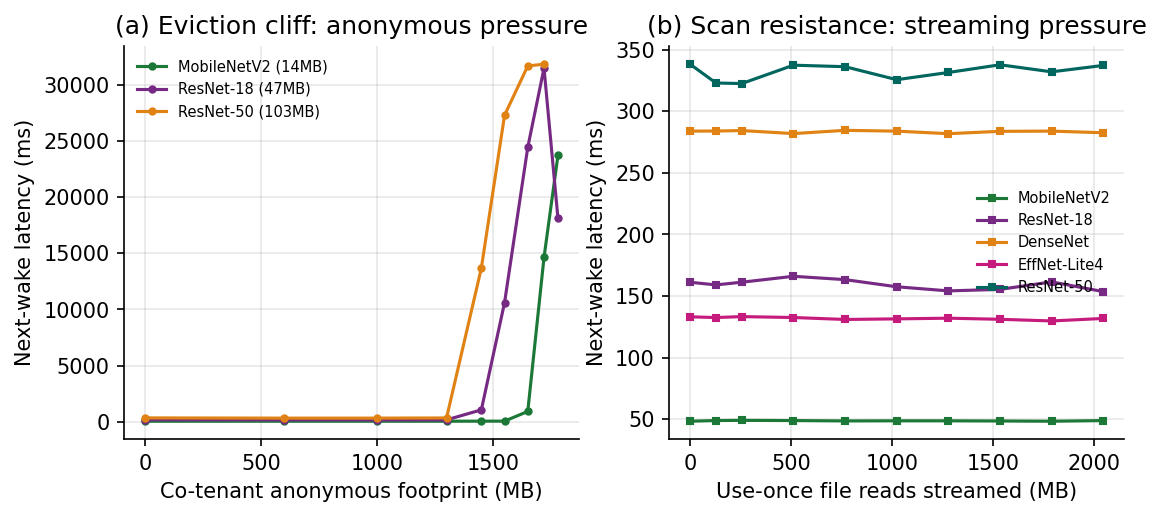
\includegraphics[width=0.95\columnwidth]{figs/fig4_cliff.png}
\caption{The eviction cliff. Anonymous co-tenant memory pressure during the idle interval evicts
the model's pages once free memory drops below its footprint, re-triggering the full cold-start
tax on the next wake. (Use-once streaming pressure, by contrast, leaves the model warm.)}
\label{fig:cliff}
\end{figure}

\section{The Energy of a Wake}\label{sec:energy}
Latency is only half the cost; for battery- and harvesting-powered devices the energy of a wake
sets the duty-cycle budget. Using the Pi~5's PMIC telemetry we measure the energy of a cold wake,
a warm wake, and a steady-state inference (Fig.~\ref{fig:energy}, Table~\ref{tab:main}). A single
cold wake costs the energy of \CINFRANGE\ steady-state inferences. \ENERGYPARA

\begin{figure}[t]\centering
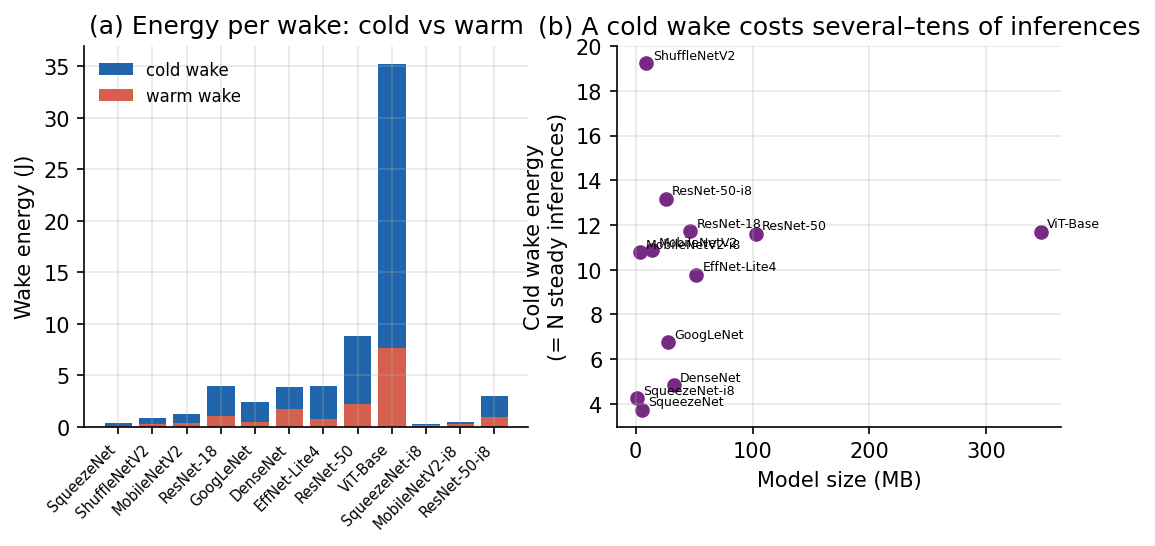
\includegraphics[width=\columnwidth]{figs/fig5_energy.png}
\caption{(a) Cold vs.\ warm wake energy per model. (b) A cold wake costs the energy of 4--19
steady-state inferences, scaling with model size.}
\label{fig:energy}
\end{figure}

\subsection{The DVFS Ramp Adds Little}\label{sec:dvfs}
Because the cold wake is dominated by flash I/O rather than computation, one might expect the
CPU clock to matter little during a wake. Figure~\ref{fig:dvfs} confirms it. Comparing the
default on-demand governor (\texttt{schedutil}), which starts near the minimum clock and ramps up
during the wake, against a pinned \SI{2.4}{GHz}, the governor's ramp adds only
\SIrange{0}{4}{\percent} to cold-wake latency (mean ${\sim}\RAMPMEAN\%$). The wake is I/O-bound,
so paying maximum-clock energy through it is largely wasted---a useful corollary given that
max-clock operation is already energetically wasteful for steady-state
inference~\cite{jacob2026energy}.

\begin{figure}[t]\centering
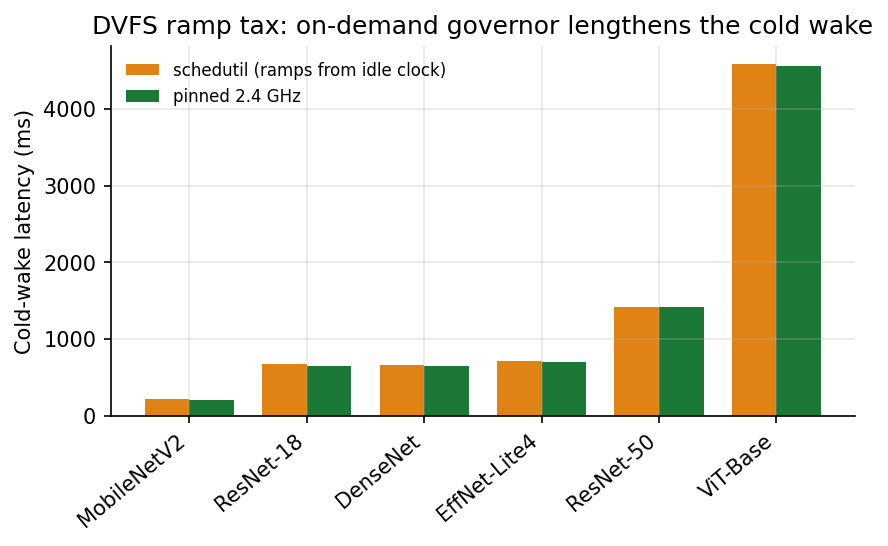
\includegraphics[width=0.95\columnwidth]{figs/fig6_dvfs.png}
\caption{DVFS ramp tax. Because the wake is I/O-bound, the on-demand governor's clock ramp adds
only a few percent to cold-wake latency over a pinned maximum clock.}
\label{fig:dvfs}
\end{figure}

\section{How Many Inferences Justify a Wake?}\label{sec:amortize}
The cold-start tax is a fixed cost per wake, amortized over the $B$ inferences the device runs
before sleeping again. Figure~\ref{fig:amortize} plots the cold-start overhead---in both time and
energy---as a fraction of the total wake, against $B$. For a device that wakes to run a single
inference ($B=1$), the overhead is essentially the entire tax: \OVERHEADBONE\ of the wake's time
and \OVERHEADBONEE\ of its energy is cold start rather than useful work. Overhead falls below
10\% only at $B=\BTENLO$--\BTENHI\ inferences per wake, depending on the model. This quantifies
the duty-cycle regime in which cold start matters: a doorbell camera classifying one frame per
event lives entirely in the tax; a device batching hundreds of inferences per wake escapes it.
The practical consequence is that \emph{the duty-cycle ratio, not the steady-state throughput,
determines whether cold start must be engineered around}.

\begin{figure}[t]\centering
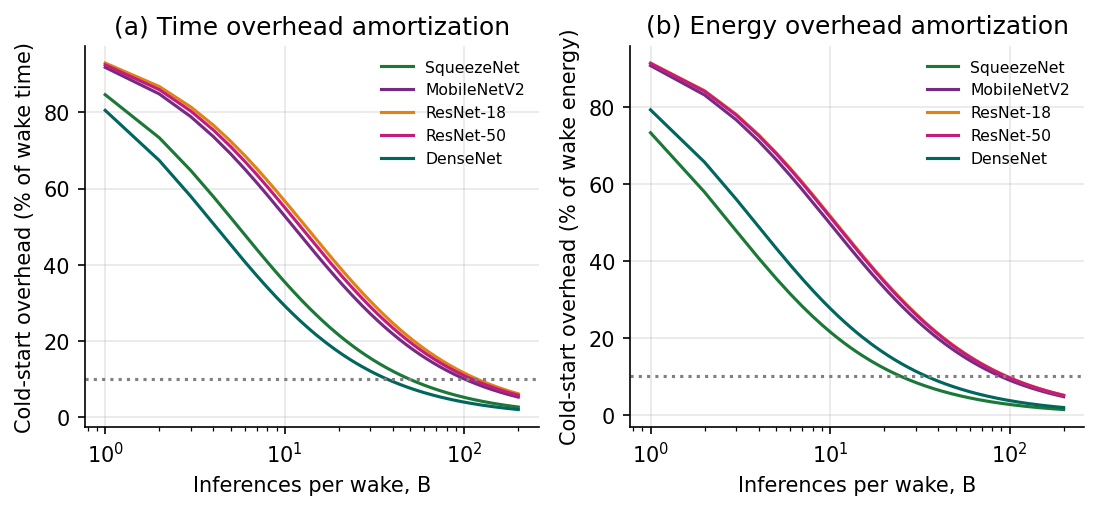
\includegraphics[width=\columnwidth]{figs/fig9_amortize.png}
\caption{Amortizing the tax. Cold-start overhead as a fraction of (a) wake time and (b) wake
energy versus inferences per wake $B$. Below $B\approx\BTENLO$--$\BTENHI$ the tax dominates.}
\label{fig:amortize}
\end{figure}

\subsection{Disable Graph Optimization for Short Wakes}\label{sec:optpolicy}
ONNX Runtime's default is to apply all graph optimizations, which speeds steady-state inference
but lengthens session creation---part of the tax. For a duty-cycled device this default can be
counter-productive. Comparing optimization levels, disabling optimization reduces cold-wake
latency (a smaller build) at the cost of slower steady inference, so there is a crossover $B^{*}$:
below $B^{*}$ inferences per wake, \emph{disabling} optimization minimizes total wake-plus-work
time. \OPTPARA\ This is a zero-cost configuration change---one enum---that directly reduces the
tax for low-duty-cycle deployments, and it composes with the residency policy below.

\section{\texorpdfstring{\gdtax}{GD-Tax}: A Tax-Aware Residency Policy}\label{sec:policy}
The measurements above imply an operating principle for multi-model edge devices: because a cold
wake costs the energy of many inferences and re-triggers whenever memory is pressured, the device
should keep \emph{warm} the sessions whose eviction would be most expensive---not simply the most
recently or most frequently used. We formalize this as cost-aware caching and evaluate it on the
measured constants.

\textbf{Problem.} A device serves a stream of requests to $K$ models but has a RAM budget $B$ too
small to hold every session warm. On a request to a resident (warm) model it pays the steady cost
$(L_s^i, E_s^i)$; on a request to an evicted model it pays the cold wake $(L_c^i, E_c^i)$ and the
model becomes resident, evicting others to fit $B$. Each resident model occupies $m_i$ MB
(measured resident footprint, 9--265\,MB). The goal is to minimize energy per request (and tail
latency) over the trace.

\textbf{Policy.} \gdtax{} is a Greedy-Dual policy~\cite{cao1997greedydual} whose retention
priority is keyed on each model's \emph{measured cold-wake energy penalty}
$\Delta E_i = E_c^i - E_s^i$: on access, model $i$'s priority is set to $H\!\leftarrow\! H_{\min}
+ \Delta E_i$, and the resident model with the smallest priority is evicted, with the classical
aging that raises $H_{\min}$ to the evicted priority. High-tax models are thus retained
preferentially, exactly in proportion to what their eviction would cost. Unlike FaasCache's
server keep-alive~\cite{fuerst2021faascache}, the cost is a measured on-device energy penalty and
the constraint is physical RAM.

\begin{algorithm}[t]
\caption{\gdtax{} residency on a request to model $i$}
\label{alg:gdtax}
\begin{algorithmic}[1]
\State \textbf{state:} resident set $R$, priorities $H$, budget $B$, aging base $L$
\If{$i \in R$} \Comment{warm hit}
  \State $H_i \gets L + \Delta E_i$ \Comment{$\Delta E_i = E_c^i - E_s^i$, measured}
  \State pay $(L_s^i, E_s^i)$
\Else \Comment{cold miss}
  \State pay $(L_c^i, E_c^i)$
  \While{$\sum_{j\in R} m_j + m_i > B$}
    \State $v \gets \arg\min_{j\in R} H_j$; \; $L \gets \max(L, H_v)$; \; $R \gets R\setminus\{v\}$
  \EndWhile
  \State $R \gets R\cup\{i\}$; \; $H_i \gets L + \Delta E_i$
\EndIf
\end{algorithmic}
\end{algorithm}

\textbf{Evaluation.} We simulate \gdtax{} against always-reload (no cache), LRU, LFU, and a
cost-aware Belady oracle~\cite{belady1966study} on the measured constants, over a Zipf popularity
workload and a detect$\rightarrow$classify pipeline workload, sweeping $B$ from 15\% to 100\% of
the all-resident footprint (Fig.~\ref{fig:policy}). \POLICYPARA

\section{Discussion and Limitations}\label{sec:discussion}
\textbf{Implications for practice.} The results argue for three changes in how edge inference is
reported and engineered. (i) \emph{Report the cold wake.} A steady-state latency/energy pair is
insufficient for a duty-cycled deployment; a cold-wake latency and energy should accompany it,
and the duty-cycle period and memory budget should be evaluation axes. (ii) \emph{Optimize
loading, not warm-up.} Because there is no compute warm-up but weight loading dominates,
effort is best spent on faster or avoided loading---keeping sessions resident, memory-mapping
weights, faster storage, or smaller files---rather than on warm-up loops. (iii) \emph{Budget for
re-warm.} On a memory-constrained device the tax recurs whenever a co-tenant's working set grows;
residency must be managed, which \gdtax{} does using the measured energy penalty as its currency.

\textbf{Generality and threats to validity.} Our measurements are ARM Cortex-A76 / ONNX Runtime /
microSD specific. The \emph{ratios} we report (tax multiple, disk-dominated decomposition, absent
compute warm-up, I/O-bound wake) should transfer to other CPU edge runtimes, but absolute values
depend on storage bandwidth (a faster NVMe or eMMC would shrink the disk term and thus the tax)
and on the runtime's graph-optimization cost. The PMIC telemetry samples at ${\sim}\SI{10}{Hz}$,
so per-wake energy for the shortest wakes is estimated from pooled power over many repetitions
rather than a single window; we report medians and anchor quantitative claims on the
well-sampled larger models. The residency policy is evaluated in simulation on measured
per-model constants and synthetic-but-realistic traces; an on-device implementation and a
field-trace evaluation are natural next steps. Finally, an accelerator (GPU/NPU) execution
provider would change the compute term but would, if anything, \emph{increase} the relative
weight of loading, strengthening the paper's thesis.

\begin{figure}[t]\centering
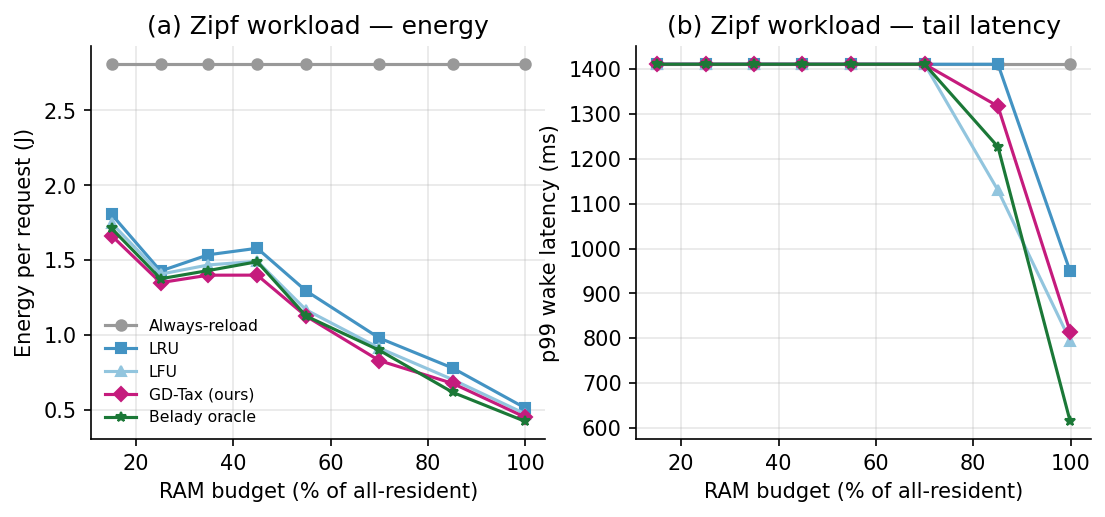
\includegraphics[width=\columnwidth]{figs/fig7_policy.png}
\caption{\gdtax{} vs.\ baselines on measured constants (Zipf workload). By retaining the
highest-energy-penalty models, \gdtax{} cuts energy per request and tail latency at tight RAM
budgets, approaching the Belady oracle and far below LRU/LFU and always-reload.}
\label{fig:policy}
\end{figure}


\section{Conclusion}\label{sec:conclusion}
Duty-cycled edge inference pays a cold-start tax that steady-state benchmarks make invisible.
On a Raspberry~Pi~5 the tax is 5--23$\times$ the steady-state latency, is dominated by loading
weights from flash rather than by any compute warm-up, costs the energy of 4--19 steady-state
inferences per wake, and re-triggers whenever a small page cache is pressured during idle. These
facts change what an edge deployment should optimize: not the hot-loop kernel, but the wake.
Our \gdtax{} residency policy is one consequence---keeping warm the sessions whose eviction would
cost the most energy---but the broader message is methodological. We recommend that edge-inference
studies report a cold-wake latency and energy alongside steady-state numbers, and that duty-cycle
period and memory budget be treated as first-class evaluation axes.

\bibliographystyle{IEEEtran}
\bibliography{refs}
\end{document}
